% Updated in February 2016 by Hwann-Tzong Chen
% Updated in May 2014 by Hideo Saito
% Updated in March 2012 by Yasuyuki Matsushita
% Updated in April 2002 by Antje Endemann, ...., and in March 2010 by Reinhard Klette
% Based on CVPR 07 and LNCS style, with modifications by DAF, AZ and elle 2008, AA 2010, ACCV 2010

\documentclass[runningheads]{llncs}
\usepackage{graphicx}
\usepackage{amsmath,amssymb} % define this before the line numbering.
\usepackage{ruler}
\usepackage{color}
\usepackage{subfigure}
\usepackage{mathrsfs}
\usepackage[marginal]{footmisc}
\renewcommand{\thefootnote}{}
\usepackage{bm}
\usepackage{booktabs}
\usepackage{array}
\newcommand{\PreserveBackslash}[1]{\let\temp=\\#1\let\\=\temp}
\newcolumntype{C}[1]{>{\PreserveBackslash\centering}p{#1}}
\newcolumntype{R}[1]{>{\PreserveBackslash\raggedleft}p{#1}}
\newcolumntype{L}[1]{>{\PreserveBackslash\raggedright}p{#1}}
%===========================================================
\begin{document}
\pagestyle{headings}
\mainmatter

\def\ACCV16SubNumber{***}  % Insert your submission number here

%===========================================================
\title{Robust Building Extraction from Large-scale Aerial Scene with Multi-scale Fully Convolutional Network} % Replace with your title
\titlerunning{ACCV-16 submission ID \ACCV16SubNumber}
\authorrunning{ACCV-16 submission ID \ACCV16SubNumber}

\author{Anonymous ACCV 2016 submission}
\institute{Paper ID \ACCV16SubNumber}

\maketitle
%===========================================================
\begin{abstract}
   \textbf{Automatic building extraction from remote sensing image plays a critical role in  a diverse range of applications. However, it is  a huge challenge to extract any-size buildings with large variational appearances and occlusions. To tackle these problems, we propose a robust system employing a improved multi-scale fully convolutional networks(MSFCNs), which effectively integrates the information generated from a group of neurons with multi-scale receptive fields. \textbf{XXXXXXXXXXXXXX}
   Our architecture can take a whole aerial images as inputs without warping or cropping and output building map directly.  The experiment results test on a publicly available aerial imagery dataset proved that our proposed  methodology significantly shorten time-consuming and surpass the performance of state-of-the-art.}

\end{abstract}

%===========================================================
\section{Introduction}
   With the rapid development of remote sensing technologies and popularization of geospatial related commercial software, very high resolution satellite images are very easily accessible, these valuable data provides a huge fuel for interpreting real terrestrial scenes. Building rooftops is one of the most important type of terrestrial objects because it is essential for a wide range of technologies, such as, urban planning, automated map making, 3D city modelling, disaster assessment, military 	reconnaissance, etc. However, it is very costly and time-consuming to manually delineate the footprint of buildings even for human experts. 
   
   In recent decades, many researchers have made massive attempts to extract buildings automatically. Much of the past of work defines criteria according to the unique  characteristics of rooftop, such as regular shapes\cite{noronha2001detection}\cite{nosrati2009novel}\cite{izadi2012three}\cite{wang2015efficient}, homogeneous color \cite{cote2013automatic}, surrounding shadows \cite{ok2013automated} 
   
    \textbf{  In this article, we aim at deploying a robust building extraction system that can handle buildings with different sizes, variational appearances and occlusions.  }
 
   The rest of this article is organized as follows. The section 2.1 outlines some key ideas of fully convolutional network(FCN), the section 2.2 provides details of our neural network architecture. In section 2.3 the formulation of our system is proposed. The section 4.1 presents the datasets which is used for training and testing in our experiments. The section 3.2  introduces training settings and strategies of our proposed network.  The section 3.3, we compare our results with two patch based methods using same dataset with us. In section 4, we discuss the experimental results and summarize whole article. 
   
   
\subsection{Related Works}
	 According to our experience of life, we learn that the most of building rooftops have more regular shapes, which usually are rectangular or combinations of several rectangles. Hereby, \cite{noronha2001detection}\cite{nosrati2009novel}\cite{izadi2012three}\cite{wang2015efficient} exploited a graph-based search to establish a set of rooftop hypotheses through examining the relationships of lines and line intersections, and then removed the fake hypotheses using a series of criteria. \cite{cote2013automatic} generated rooftop outline from selected corners in  multiple color and color-invariance spaces, further refined to fit the best possible boundaries through level-set curve evolution. Though these geometric primitives based methods methods achieve good performance in high contract remote sensing imagery , they suffer from three serious shortcomings. Firstly, they lack the ability of detecting arbitrarily shaped building rooftop. Secondly, they fail to  extract credible geometric features in buildings with inhomogeneous color distribution or low contrast with surroundings. Thirdly, it is hardly possible to process large-scale scenes because of their high computational-complexity.	
	
   Apart from using shape information, spectral features is a distinctive feature for  terrestrial object detection. For instance, shadows are commonly dark grey or black, vegetations are usually green or yellow with particular textures, and main roads are dim gray with different road marks in most case. According to these prior knowledge, Ghaffarian \textit{et al.} \cite{ghaffarian2014automaticPFICA} split aerial scene into three components(respectively, shadows and the vegetation, roads and the bare soil, building) using a group of manually set rules. Afterwards, a purposive fast independent component analysis (PFastICA) technique is employed to separate building area from remote sensing image. However, the results is significantly sensitive to parameter choice. A feasible alternative strategy is to learn the appearance representation using  supervised learning algorithm. \cite{chen2014shadow}\cite{dornaika2015object}\cite{baluyan2013novel}\cite{ngoautomatic} designed a similar framework. Firstly, aerial image is divided into superpixels using  a certain over-segmentation algorithm. Secondly, hand-craft features, such as, color histograms or local binary patterns, are extracted from each over-segmented regions. Finally, each region was classified using machine learning tools and a gallery of training descriptors. \textbf{ Because it's inevitable for machine learning method to mislabel regions with close appearance, additional information is utilized to refine previous result.} \cite{ngoautomatic} removed false rooftops using a assumption that buildings are surrounded by shadows because of illumination. \cite{baluyan2013novel} devised a ``histogram method" to detect missed rooftops. \cite{li2015robust} select probable rooftops after pruning out blobs using shadows, light direction, a series of shape criteria, and then these rooftops is refined by high order conditional random field. The drawbacks are threefold. (1) It is problematic to recognize a over-segmented region as building because terrestrial objects have huge variational appearance in real aerial scene. (2) Hand-craft features are not robust to large-scale remote sensing image. (3) Additional information is unreliable. For instance, some buildings have no shadow in its neighbourhood, and some buildings have unique structures which are not satisfied to hand-coded criteria. 

    As mentioned above, traditional methods are not capable of adapting to real scenes with huge variational appearance, occlusion and low contrast. Recently, deep neural networks have been widely deployed in general image segmentation or scene labelling tasks. Mnih, a pioneer, have presented a patch-based framework in \cite{Mnih2013Machine} for learning to label aerial images. A  neural network architecture is carefully designed for predicting buildings in aerial imagery, and then the output of this network is processed by conditional random fields(CRFs). Satito \cite{Saito2016Multiple} improved Mnih's networks for extracting multiple kinds of objects simultaneously, two techniques consisting of model averaging with spatial displacement(MA) and channel-wise inhibited softmax (CIS) are introduced to enhance the  performance. However, both two methods need to crop test image into a fixed size, which not only increase the time loss, but also break the integrity of building. For example, they obtain bad performance for large-size or occluded buildings (see Fig. \ref{fig:BadResults}) and cost about 9s for 1500 $\times$ 1500 image without model averaging. 
   
   Mapping buildings from aerial image is essentially a problem of semantic segmentation. Recent work suggests a number of methods in processing natural images.  Chen et al. \cite{chen14semantic} present a system which combine the responses at the final convulotional layer with a fully connected conditional random field (CRF). The system is able to localize segment boundaries at a quite high level of accuracy. An end-to-end network \cite{Zheng2015Conditional}  which integrates CRF modelling with CNNs avoids off-line post-processing methods for object delineation. Noh et al. \cite{Noh2015Learning} apply a deconvolution network to each proposal in an input image, and construct the final semantic segmentation map by combining the results from all proposals in a simple manner.
     
   Although these methods show promise in segmenting natural images, they have components not suited for building extraction. First, buildings are frequently occluded by shadows or trees (see Fig.\ref{fig:AerialImages} (a)). It is challengable to delineate building boundaries even for human experts. \textbf{Though \cite{chen14semantic} \cite{Zheng2015Conditional} achieve excellent performance in processing boundary of natural image, neither of them reported that they have strong ability to handle occlusions.}
Second, buildings have significantly variational appearance even in a single one. (see Fig.\ref{fig:AerialImages} (b)). Moreover, a number of buildings are very close to the plot on the ground or road (see Fig.\ref{fig:AerialImages} (c)). Based on our observation, there are few samples emerged in PASACAL VOC 2012 dataset. Last but not the least, the size of objects in a remote sensing image is in a wide range. For example, some images include a large number of tiny buildings (see Fig.\ref{fig:AerialImages} (d)) and some ones are composed of moderate quantity of small-scale rooftops and a few of large-scale rooftops. \cite{Noh2015Learning} claimed that it handles objects in multiple scales, but it only suitable to multi-class object segmentation. 

\begin{figure}
\centering
\label{fig:AerialImages}
\includegraphics[width=120mm]{AerialImages}
\caption{Examples of aerial image}
\end{figure}

%===========================================================
\section{Proposed Method} 
    In this section, we firstly introduce a well-known semantic segmentation network, called fully convolutional network(FCN)\cite{Long2014Fully}. We attempt to extract footprints of building  using  architecture proposed by author and two modified versions. Our experiments show that these networks are not enough to accomplish building  extraction task. \textbf{Inspired by \cite{Xie2015Holistically}, we introduce a multi-scale fully convolutional network(MSFCN) for extracting rooftops, it turns out to be achieve state-of-the-art performance in a public aerial image dataset.} Finally, we formulate our problem and loss function.
         
\subsection{Fully Convolutional Network}
    As mentioned in introduction, patch-based building extraction methods \cite{Mnih2013Machine} \cite{Saito2016Multiple} suffer from shortcoming in processing big buildings because of the fixed-size inputs. As far as we know, fully convolutional network(FCN) takes whole image as inputs and directly outputs building rooftops by one pass of forward propagation. Because it can process input images of any sizes without warping or cropping, integrality of object is protected much better. 
	
	Long \textit{et al.} put forward the concept of fully convolutional network(FCN) in \cite{Long2014Fully} for the first time. \textbf{It said: ``While a general deep net computes a general nonlinear function, a net with only layers of this form computes a nonlinear filter, which we call a deep filter or fully convolutional network.''} In practice, the fully connected layers in traditional CNNs are transformed to convolutional layers with 1 $\times$ 1 kernels. Due to the mechanism of pooling, the output of the network is a coarse heat map. For pixelwise prediction, skip-net technique is used to connect various coarse outputs back to pixels. For example, the framework of FCN-8s is described as following. We firstly obtain the 16 stride predictions by fusing the predictions of pooling4 with the 2 $\times$ upsampling of predictions from \textit{conv7}(convolutionalized \textit{fc7}). Then we continue in this fashion by fusing predictions from \textit{pool3} with a 2 $\times$ upsampling of the 16 stride predictions, denoted as 8 stride predictions. Finally, the 8 stride predictions are upsampled back to image with original size. 
	 
	In our experiments, we first directly apply the FCN-8s to extract building rooftop by replacing the loss function with sigmoid cross-entropy loss. In order to achieving better performance, the network is extended to FCN-4s, FCN-2s. Our experiments show that FCN-4s and FCN-2s get the best performance with overall recall of 70.19 $\%$ in precision recall breakeven point. According to our results, the first row of Fig. \ref{fig:FCN4s-results} indicates that FCN-4s has less ability to handle  objects with small size. The second row of Fig. \ref{fig:FCN4s-results} shows that it is hard for FCN to discriminate buildings with ground if their color is similar. To overcome these drawbacks, a improved FCN is introduced in next section. 
	
\begin{figure}
\centering
\subfigure[]{	
	\label{fig:InputImage}
	\includegraphics[width=35mm]{FCN4s-results-Input(a)}}
\subfigure[]{
	\label{fig:GroundTruth}
	\includegraphics[width=35mm]{FCN4s-results-GT(b)}}
\subfigure[]{
	\label{fig:FCN-4s}
	\includegraphics[width=35mm]{FCN4s-results-Prediction(c)}}
\subfigure[]{	
	\label{fig:InputImage}
	\includegraphics[width=35mm]{FCN4s-results-Input(d)}}
\subfigure[]{
	\label{fig:GroundTruth}
	\includegraphics[width=35mm]{FCN4s-results-GT(e)}}
\subfigure[]{
	\label{fig:FCN-4s}
	\includegraphics[width=35mm]{FCN4s-results-Prediction(f)}}
\caption{(a)(d) Input image. (b)(e) Ground truth. (c)(f) FCN-4s prediction.}
\label{fig:FCN4s-results}
\end{figure}
 
\subsection{Our Architecture} 
   There are three reasons that FCN-8s is not appropriate methods for building extraction. (1) \textbf{The output of 32 stride layers, including convolutionalized \textit{fc6, fc7} and fifth pooling layer, is too fuzzy to utilize. Meanwhile, the neurons numbers of convolutionalized \textit{fc6, fc7} are too large to cost intensive computation.} (2) The output from FCN-8s is at one-eight of the input resolution. It is not dense enough for very high resolution remote sensing image. Though FCN4s and FCN2s can increase the resolution, they have little help for improving performance. Defective fusion strategy is the most likely reason. On the one hand, in \cite{Long2014Fully}, the coarse predictions from a late stage are upsampled and combined with prediction from its preceding stage using simple sum operation. (3) \textbf{In ConvNet, the latter the layer is, the less the spatial information is and the richer the semantic information is. For instance, in FCN-8s, the firth stage generate low level semantic information, such as, regions with similar color or texture, and fine spatial resolution. On the contrary, the last stage outputs strong semantic features but coarse map.} FCN-8s takes no account of combining semantic information and spatial information effectively.  
  
%   \begin{table}
%	\label{tab:receptivefield} 
%	\centering
%	\caption{The receptive field and stride size in VGG16 net. Bolded layer is used in our architecture.}	
% 	\begin{tabular}{C{1cm}|*{16}{C{0.74cm}}} 
%	\hline
%	layer & $\bm{c1\_1}$ & $\bm{c1\_2}$  & $\bm{c2\_1}$  & $\bm{c2\_2}$  & c3$\_$1  & c3\_2  & $\bm{c3\_3}$  & c4$\_$1}  &   c4$\_$2  & $\bm{c4\_3}$  & c5$\_$1} & c5$\_$2  & $\bm{c5\_3}$ \\
%	\hline
%    rf size & $\bm{3}$ & $\bm{5}$  & $\bm{10}$  & $\bm{14}$  & 24  & 32  & $\bm{40}$  & $\bm{60}$  & 76  & $\bm{92}$  & $\bm{124}$  & 164  & $\bm{196}$ \\
%	\hline
%	stride & $\bm{1}$ & 1   & $\bm{2}$  & 2  & $\bm{4}$  & 4  & $\bm{4}$  & $\bm{8}$  & 8  & $\bm{8}$  & $\bm{16}$  & 16  & $\bm{16}$ \\
%	\hline
%    \end{tabular}
%   \end{table}   
   
   Based on the above analysis, we therefore make the following modifications: (1) Convolutionalized \textit{fc6, fc7} and fifth pooling layer are cut. (2) We design three  selection modes to select part or all convolutional layers with incremental receptive fields (see Table \ref{tab:receptivefield}) in VGG16 net. In first mode (denote as 5-convs), for each stage, the convolutional layer with largest receptive field is chosen, receptively,\textit{ conv1$\_$2, conv2$\_$2, conv3$\_$1, conv3$\_$3, conv4$\_$1, conv4$\_$3, conv5$\_$1, conv5$\_$3}. In second mode (denote as 7-convs), for the sake of preserving spatial information,\textit{ conv1$\_$1} and \textit{conv2$\_$1} are added. In third mode (denote as 16-convs), all convolutional layer are selected. The performance of these modes will be evaluated in experiment part. These three networks are shown in Fig.\ref{fig:ThreeFuseModes}. For each selected convolutional layer, the top of which add a additional convolutional layer with 1 $\times$ 1 kernel, denoted as side outputs. (3) All side outputs are upsampled to the same size of input. Upsampling is implemented via deconvolution which is initialized by bilinear interpolation. Upsampled features maps are staked and fed into a convolutional layer with 1 $\times$ 1 kernel to yield final output. 
   
  \begin{table}
	\label{tab:receptivefield} 
	\centering
	\caption{The receptive field and stride size in VGG16 net. Bolded layer is used in our architecture.}	
 	\begin{tabular}{C{1cm}|*{16}{C{0.74cm}}} 
	\hline
	layer & $c1\_1$ & $c1\_2$  & $c2\_1$  & $c2\_2$  & $c3\_1$  & $c3\_2$  & $c3\_3$  & $c4\_1$  &   $c4\_2$  & $c4\_3$  & $c5\_1$ & $c5\_2$  & $c5\_3$ \\
	\hline
    rf size & 3 & 5  & 10 & 14  & 24  & 32  & 40  & 60  & 76  & 92 & 124  & 164  & 196 \\
	\hline
	stride & 1 & 1   & 2  & 2  & 4  & 4  & 4  &8  & 8  & 8  & 16  & 16  & 16 \\
	\hline
    \end{tabular}
   \end{table}      
   
\begin{figure}
\centering
\includegraphics[width=100mm]{ThreeFuseModes}
\caption{Our three kinds of network architectures. The first row is five stages of VGG16 net, the second row is 16-convs, the third row is 7-convs, the fourth row is 5-convs.}
\label{fig:ThreeFuseModes}
\end{figure}

\subsection{Formulation}
   Our goal is to predict probabilistic label image $\mathbf{M}$ from an input aerial image $\mathbf{S}$. Fig \ref{fig:ResultsofDifferentSupervision} shows an example of $\mathbf{S}$ and $\mathbf{M}$. We directly learn a mapping from raw pixels in $\mathbf{S}$ to a true label image  $\mathbf{M}$ by training the whole network. Here we formulate our approach for building extraction. We denote our input training data set by $\mathbf{I} = \{(\mathbf{S}_{n},\mathbf{M}_{n}),n = 1,\ldots,\vert \mathbf{S}_n \vert \}$, where sample $\mathbf{S}_{n} = \{s_{j}^{(n)}, j = 1,\ldots,\vert \mathbf{S}_n \vert \}$ denotes the raw input image and  $\mathbf{M}_{n} = \{m_{j}^{(n)}, j = 1,\ldots,\vert \mathbf{S_n} \vert\}$, $m_j^{(n)} \in \{0,1\}$ denotes the corresponding ground truth binary labelling map for satellite image $\mathbf{S}_{n}$.  Taking account of each image holistically and independently, thus, we adopt the subscript $n$ for notational simplicity. Our goal is to have a network that learns features from which it is possible to produce building maps approaching the ground truth. 
    In our image-to-image training, the loss function is computed over all pixels in a training image $\mathbf{S} = \{s_{j}, j = 1,\ldots,\vert \mathbf{S} \vert\}$ and building map $\mathbf{M} = \{m_{j}, j = 1,\ldots,\vert \mathbf{S} \vert\}$, $m_j \in \{0,1\}$.
For simplicity, we denote the collection of all standard network layer parameters as $\mathbf{W}$. For each pixel $j$ in a training image, the possibility that assigns it to building is denoted as $\hat{m}_j = Pr(m_j = 1|\mathbf{S};\mathbf{W})$. the definition of sigmoid cross-entropy loss function is shown in Eq (\ref{loss}).
\begin{equation}
	\label{loss}
    \mathcal{L} = - \frac{1}{\vert \mathbf{S} \vert} \sum_{j \in \mathbf{S}} \left[ m_j \log{\hat{m}_j} + (1 - m_j)\log{(1 - \hat{m}_j)} \right]
\end{equation}

%===========================================================
\section{Experiments}
In this section, we discuss our detailed implementation and report the performance of our proposed algorithm.

\subsection{Dataset}
   In our experiments, we use \textit{Massachusetts Buildings Dataset} (Mass. Buildings) proposed by Mnih \cite{Mnih2013Machine} and publicly available on website http://www.cs.toronto.e
du/~vmnih/data/. The dataset consists of 151 aerial images of the Boston area, with each of the images being 1500 $\times$ 1500 pixels for an area of 2.25 square kilometers. Hence, the entire dataset covers roughly 340 square kilometers. The data is split into a training set of 137 images, a test set of 10 images and a validation set of 4 images. To train the network, we create image tiles for train and validation by means of cropping entire image using a sliding window with size of 256 $\times$ 256 pixels and stride of 64 pixels. When scanning the whole dataset, image tiles with too many white pixels are removed. \textbf{After scanning, train and validation dataset include 75938 tiles and 2500 tiles with corresponding building masks}. For testing, we use ten 1500 $\times$ 1500 entire images covering area excluded from the training data. \textbf{In our experiments, we find that it is benefit for prediction to scale input image into range of [0,1]. }

\subsection{Implementation}
   The implementation of our networks are based on the publicly  available \textit{Caffe} \cite{Jia2014Caffe} Library. These three networks are fine-tuned from an initialization with the pre-trained VGG16 net model and trained in an end-to-end manner. All of our networks are trained using stochastic gradient descent with same hyper-parameters, including mini-batch size (18), initial learning rate ($10^{-5}$), learning rate is divided by 10 for each 5000 iterations, momentum (0.9), weight decay ($5\times 10^{-3}$), clip$\_$gradients (10000), number of training iterations (12000). We find that learned deconvolutions provide no noticeable improvements in our experiments, therefore,  $lr_mult$ is set to zero for all deconvolutional layers. It takes about six hours to train a network on a single NVIDIA Titan 12GB GPU.

\subsection{Our Results}
   
   
\subsection{Comparison}   
   
    \begin{table} \label{tab:PerformanceComparision}
    \centering
	\caption{Performance comparision with another methods. Recall here  means recall at breakeven. Time is computed in a single computer.}
	\begin{tabular}{L{4.1cm}C{2.6cm}C{2.6cm}C{2.2cm}}    % |c|c|c|   |表示列线
	\toprule
	& Recall(relax = 3) & Recall(relax = 0)& Time(s)\\
	\midrule
	Mnih-CNN & 0.9150 &  & \\
	Mnih-CNN + CRF & 0.9211&  & \\
	Saito-single-channel-MA & 0.9426 & & \\
	Saito-multi-channel-MA-CIS & 0.9488 & & \\
	Ours(16-convs) & $\bm{}$ & $\bm{}$ & $\bm{}$\\
	\bottomrule
	\end{tabular}
	\end{table}
 
\begin{figure}
\centering
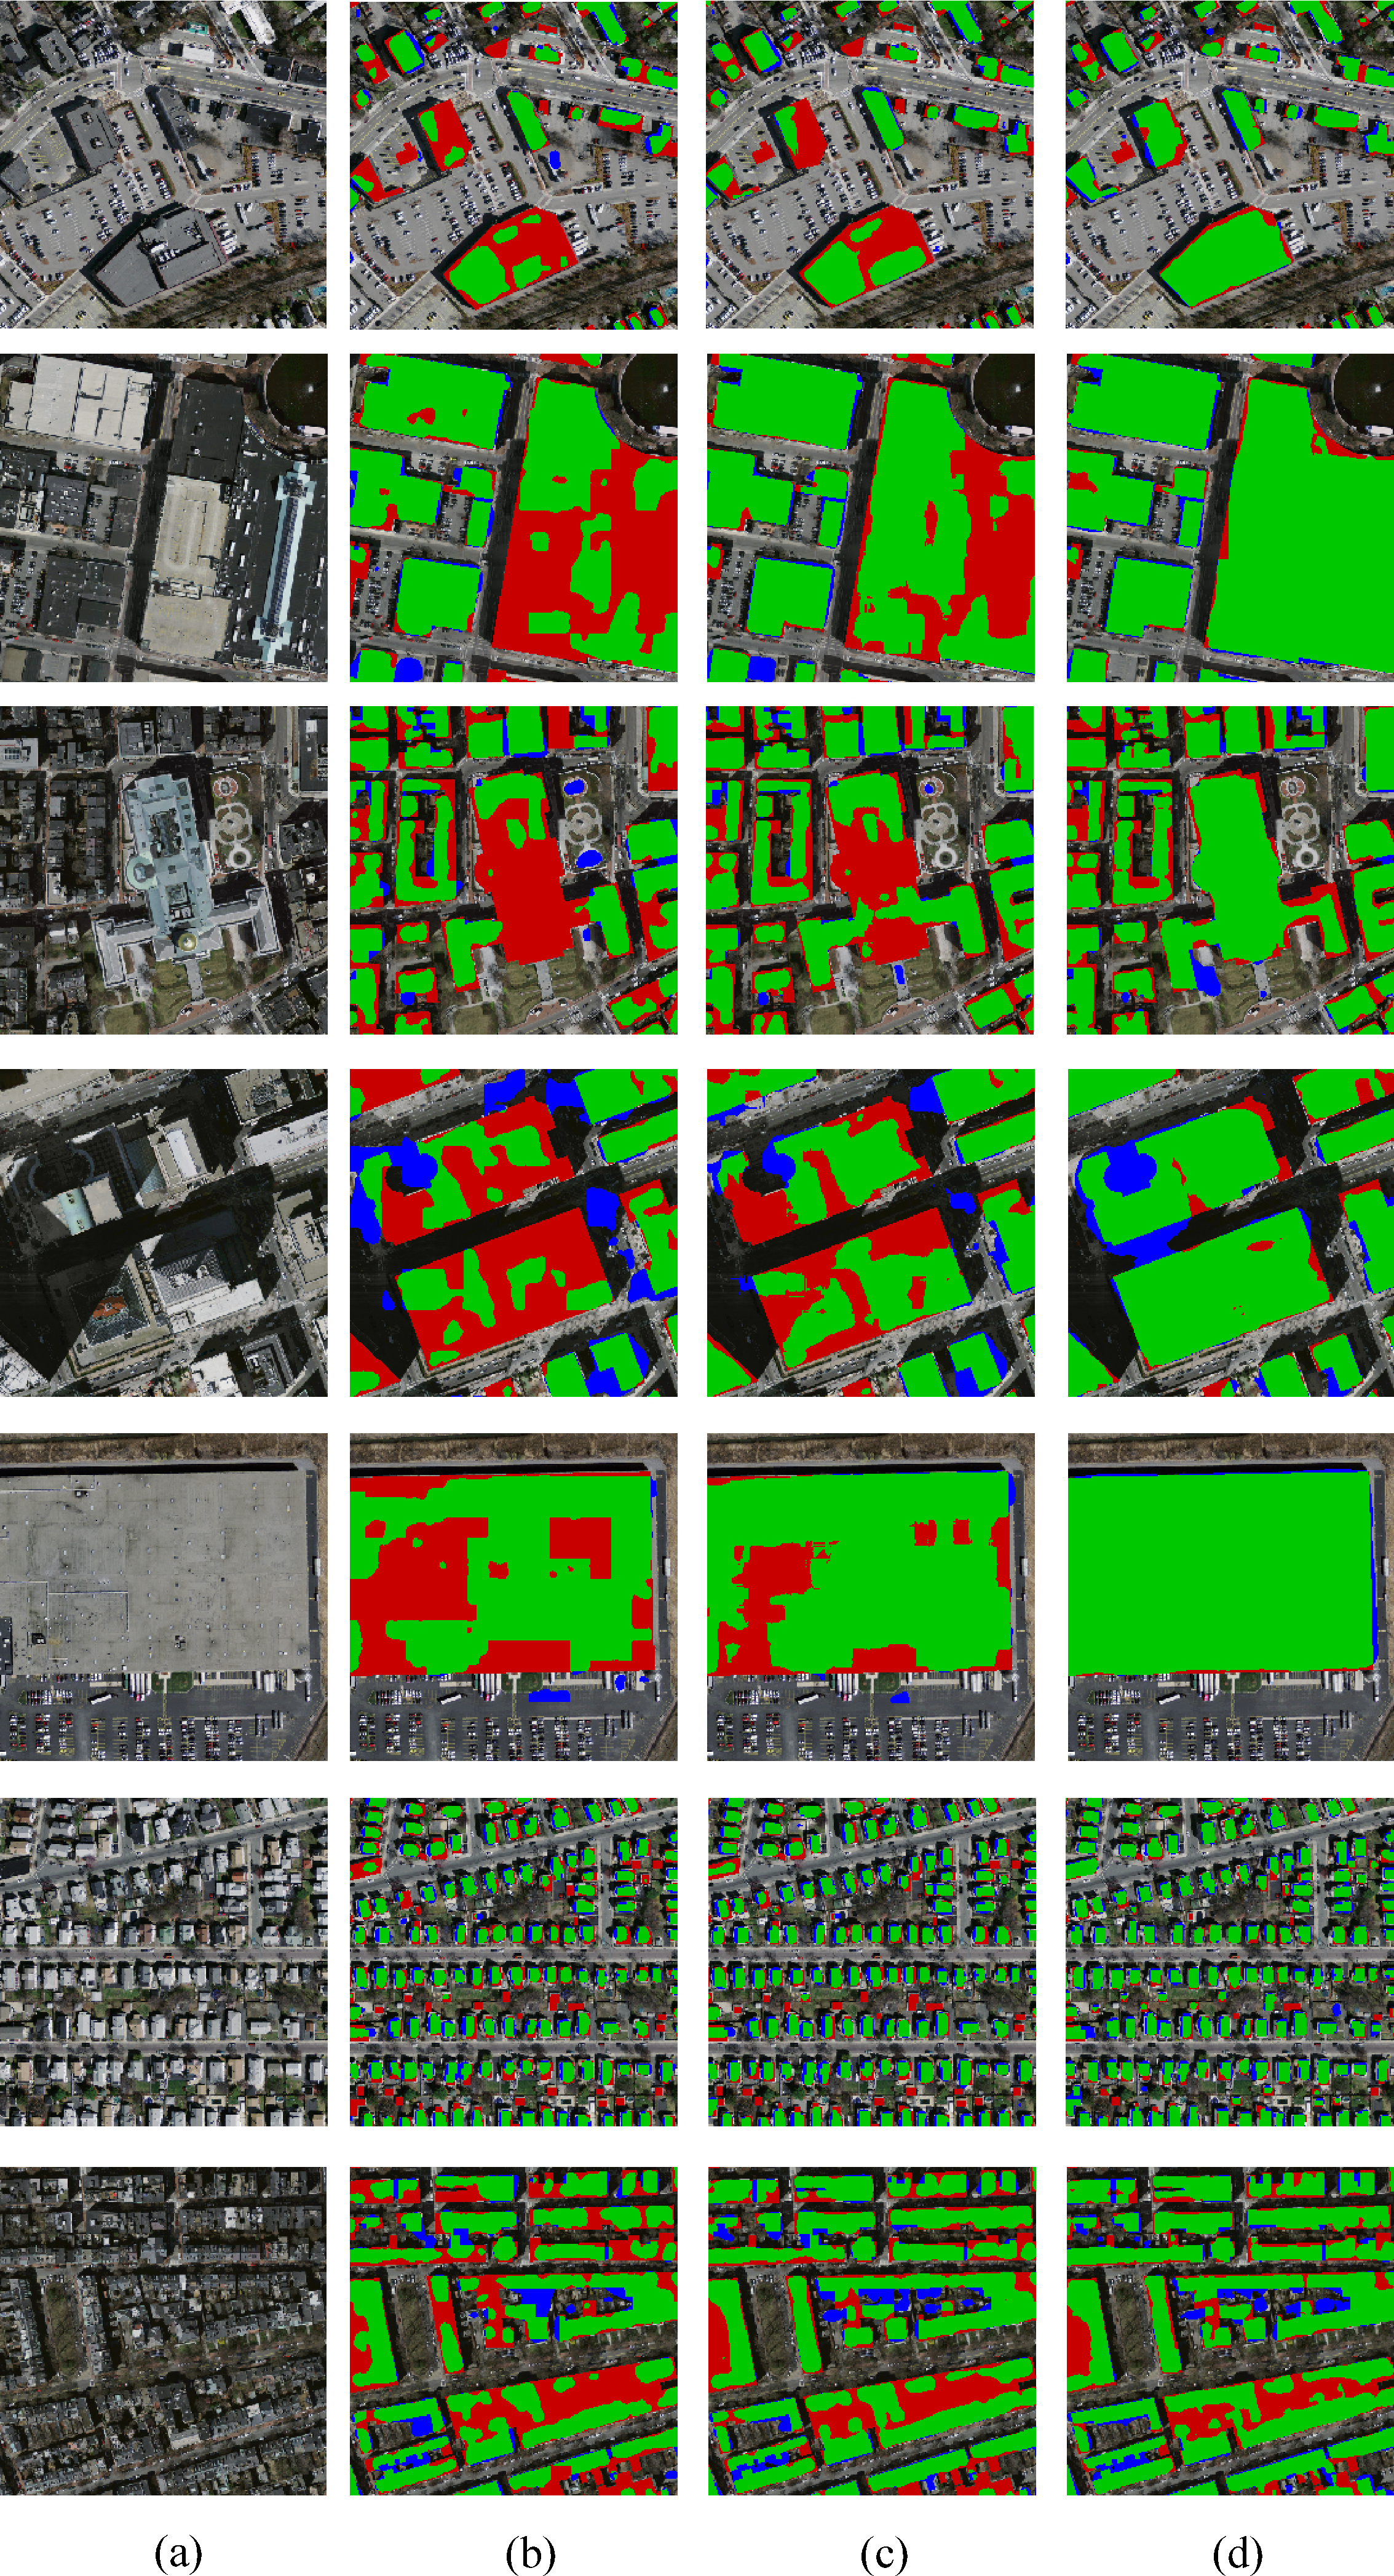
\includegraphics[width=110mm]{ComparedResults}
\caption{(a) Input image. (b) Ground Truth. (c) Mnih's result. (d) Saito's result}
\label{fig:BadResults}
\end{figure}

%===========================================================
\section{Conclusions}


%===========================================================
\bibliographystyle{splncs}
\bibliography{egbib}

%this would normally be the end of your paper, but you may also have an appendix
%within the given limit of number of pages
\end{document}
